\documentclass{article}
\usepackage{float}
\usepackage{graphicx}
% if you need to pass options to natbib, use, e.g.:
% \PassOptionsToPackage{numbers, compress}{natbib}
% before loading nips_2017
%
% to avoid loading the natbib package, add option nonatbib:
% \usepackage[nonatbib]{nips_2017}

\usepackage{nips_format}

% to compile a camera-ready version, add the [final] option, e.g.:
% \usepackage[final]{nips_2017}

\usepackage[utf8]{inputenc} % allow utf-8 input
\usepackage[T1]{fontenc}    % use 8-bit T1 fonts
\usepackage{hyperref}       % hyperlinks
\usepackage{url}            % simple URL typesetting
\usepackage{booktabs}       % professional-quality tables
\usepackage{amsfonts}       % blackboard math symbols
\usepackage{nicefrac}       % compact symbols for 1/2, etc.
\usepackage{microtype}      % microtypography

\title{Writer Identification from Handwriting}

% The \author macro works with any number of authors. There are two
% commands used to separate the names and addresses of multiple
% authors: \And and \AND.
%
% Using \And between authors leaves it to LaTeX to determine where to
% break the lines. Using \AND forces a line break at that point. So,
% if LaTeX puts 3 of 4 authors names on the first line, and the last
% on the second line, try using \AND instead of \And before the third
% author name.


\author{
  Ajinkya Rajendra Gawali
  University at Buffalo\\
  Buffalo , NY 14221 \\
  \texttt{ajinkyar@buffalo.edu} \\
  %% examples of more authors
   \And
  Juilee Paranjpe
  University at Buffalo\\
  Buffalo , NY 14221 \\
  \texttt{juileepa@buffalo.edu} \\
 } 
\begin{document}
% \nipsfinalcopy is no longer used

\maketitle

\begin{abstract}
   A decade ago, Handwriting recognition was a very difficult task but now due advancements in Machine Learning and access powerful computing power , it has become a simple toy problem. Identifying character in a handwritten text is quite easily doable but the problem that we are tackling is slightly different, we try to identify the writer given two handwritten texts, by comparing them through a machine learning model whether they belong to the same writer or not. We can test this for multiple known writers. We chose three domains of machine learning to compare and solve this problem. We first use a Multinet to get log likelihood ratio of the features being from the same writer.Secondly we used a SIFT feature extractor and Siamese Network.
   Finally we used a modern approach to solve this problem which is Deep Siamese Network.
\end{abstract}

\section{Introduction}
 In this project we use the AND DATASET which has two forms , one with human-engineered features and other with images of hand-written text 'and'. We use the human engineered features to build our two Bayesian Networks where one would represent the two features are from the same writer and the other would represent they are from diffrent writer. Using this knowledge of probability obtained from Bayesian Networks we can find out whether the two features belong to handwriting of the same writer or not.

\section{PGM}
    In this approach,we try to predict whether a given sample pair belongs to the same writer or different writer using Probablistic Graphical Model, specifically a Bayesian Network Model also known as Belief Network. Bayesian Networks are DAG's used to represent knowledge of a uncertain domain using parameters of the domain. Each node in the network is a random variable and edges represent conditional dependencies and in essence capture the causal relations between each node.For a given set of random variables their joint probablity can be calculated using a Bayesian Network using a factorization of the Bayesian Network.
    
\subsection{Dataset}
    The dataset used for this approach is in the form of features extracted by the human experts. For each handwriting sample there are 9 features that define the characteristics of that sample such as initial stroke,number and shape of arches. There are total 1026 writers and total 3524 handwritten samples whose features are provided. 
    From this dataset we are creating 1581 positive pair samples(pairs in which both samples belong to the same writer) and 5000 negative pair samples(pairs in which each sample belongs to different writer).
    \subsubsection{Positive Pair Generation}
        For a writer we take two feature vectors in the dataset where the writer id are the same.Once first feature vector is chosen the other one is chosen at random to avoid choosing the exactly same feature vector twice.This is done for all writers.
    \subsubsection{Negative Pair Generation}
        We chose a writer and then we choose another different (ID must be different) writer,We take any two feature vectors from these two writer as negative pair. We do this for all writers.
\subsection{Approach}
    \paragraph{Multinet:\\}
    Bayesian networks offer a compromise between the two
    extremes by encoding independence when possible and
    dependence when necessary. They allow a wide spectrum
    of independence assertions to be considered by
    the model builder so that a practical balance can be established
    between computational needs and adequacy
    of conclusions.[5] When the independence relations change wrt certain parameters then just single bayesian network fail to represent both independencies properly i.e single bayesian network can not handle asymmetric  independencies.\\\\
    So we use two bayesian networks to capture the variation in dependencies wrt a single pararmeter(hypothesis)
    In our case we will have one Bayesian network of 18 nodes where each node is a variable of the feature vector of a writer since there are two writers we will have 18 random variables. This Bayesian Network will be formed under the hypothesis that the 18 features belong to the same writer.
    The other Bayesian network will be formed using the hypothesis that the 18 features(9 from writer1 and 9 from writer2 ) are from different writer.\\\\
    Joint Probability can be calculated using the product of the conditional probablity distribution of each node.
    The joint probablity of 18 variables from both Bayesian networks would give the probabilty of the 18 values being from the same writer and different writer. The log of the ratio of these probablities will give us the log likelihood ratio.
\subsection{Implementation}
    For implementation of PGM approach, we have used pandas and pgmpy. We are using \textit{pandas.DataFrame} to group all positive pairs in one dataframe and all negative pairs in another.These dataframes have 18 columns such that first 9 columns represent the features of first image whereas the remaining represent the features of second  image.
    
    There are 2 broad techniques for structure learning, constraint based structure learning and score based structure learning. Content based structure learning is more useful when using some hypothesis tests, one can identify the dependencies in the structure and use these dependencies to construct Bayesian network. Since there are no hypothesis tests that can identify dependencies in gives dataset, we will use score based estimation techniques.
    
    To get the Bayesian network, we have used 3 different types of score based estimators,Bdeu Score, BIC score, K2 score.
    
    \paragraph{Bdeu Score:}
    Bdeu score stands for Bayesian Dirichlet equivalent uniform score.The scores take on the most adversary and the most beneficial priors among those within a contamination set around the symmetric one.\ [1]
    \begin{figure}[h]
  \begin{minipage}{0.48\textwidth}
  \centering
  %\fbox{\rule[-.5cm]{0cm}{4cm} \rule[-.5cm]{4cm}{0cm}}
  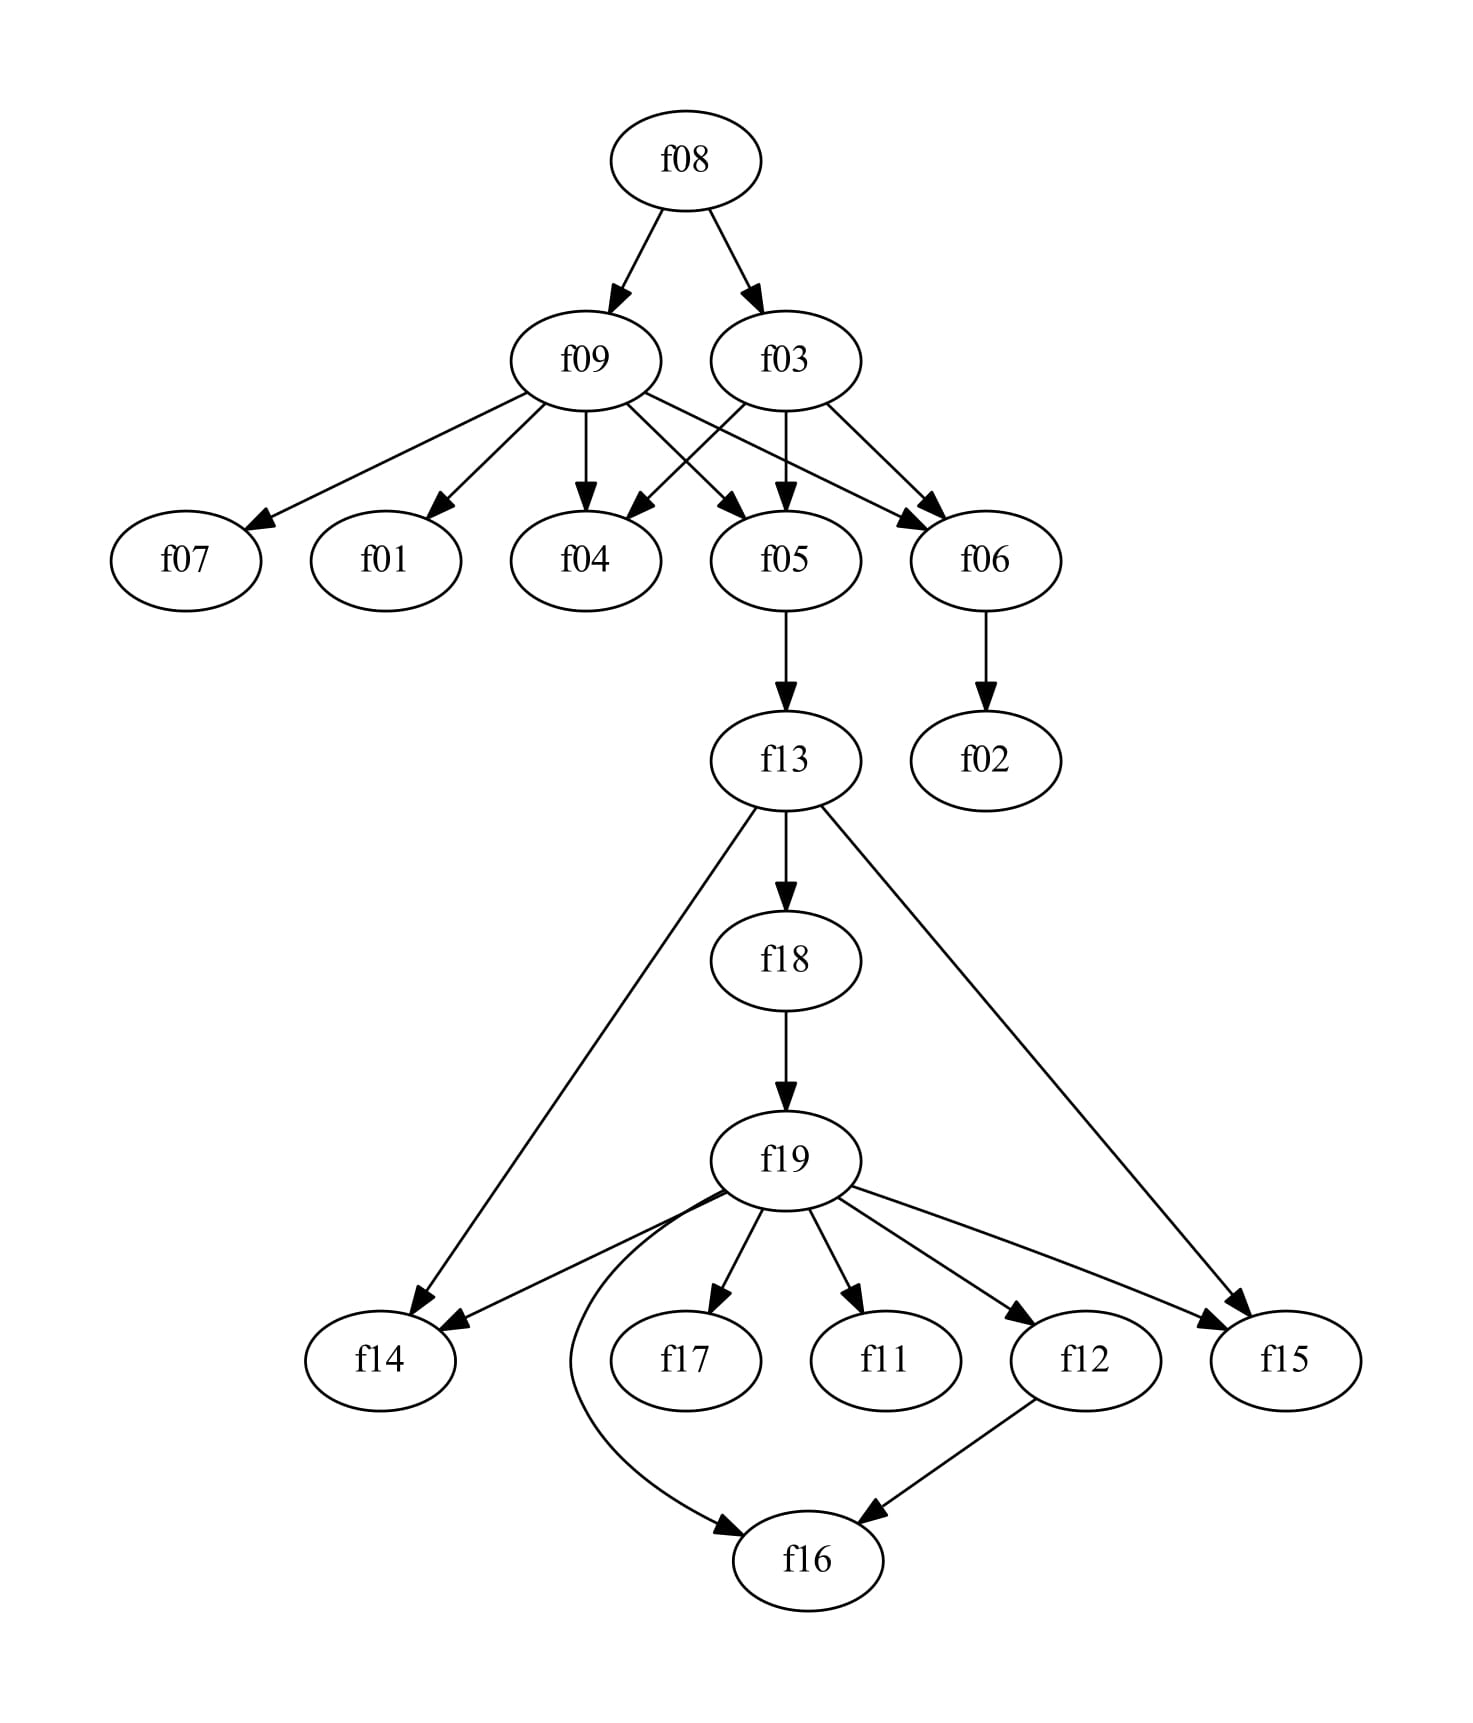
\includegraphics[width=50mm,scale=0.5]{bayesian_yes_Bdeu.jpg}
  \caption{Bayesian Network for Same Writer (BDeu Score)}
  \end{minipage}\hfill
  \begin{minipage}{0.48\textwidth}
  \centering
  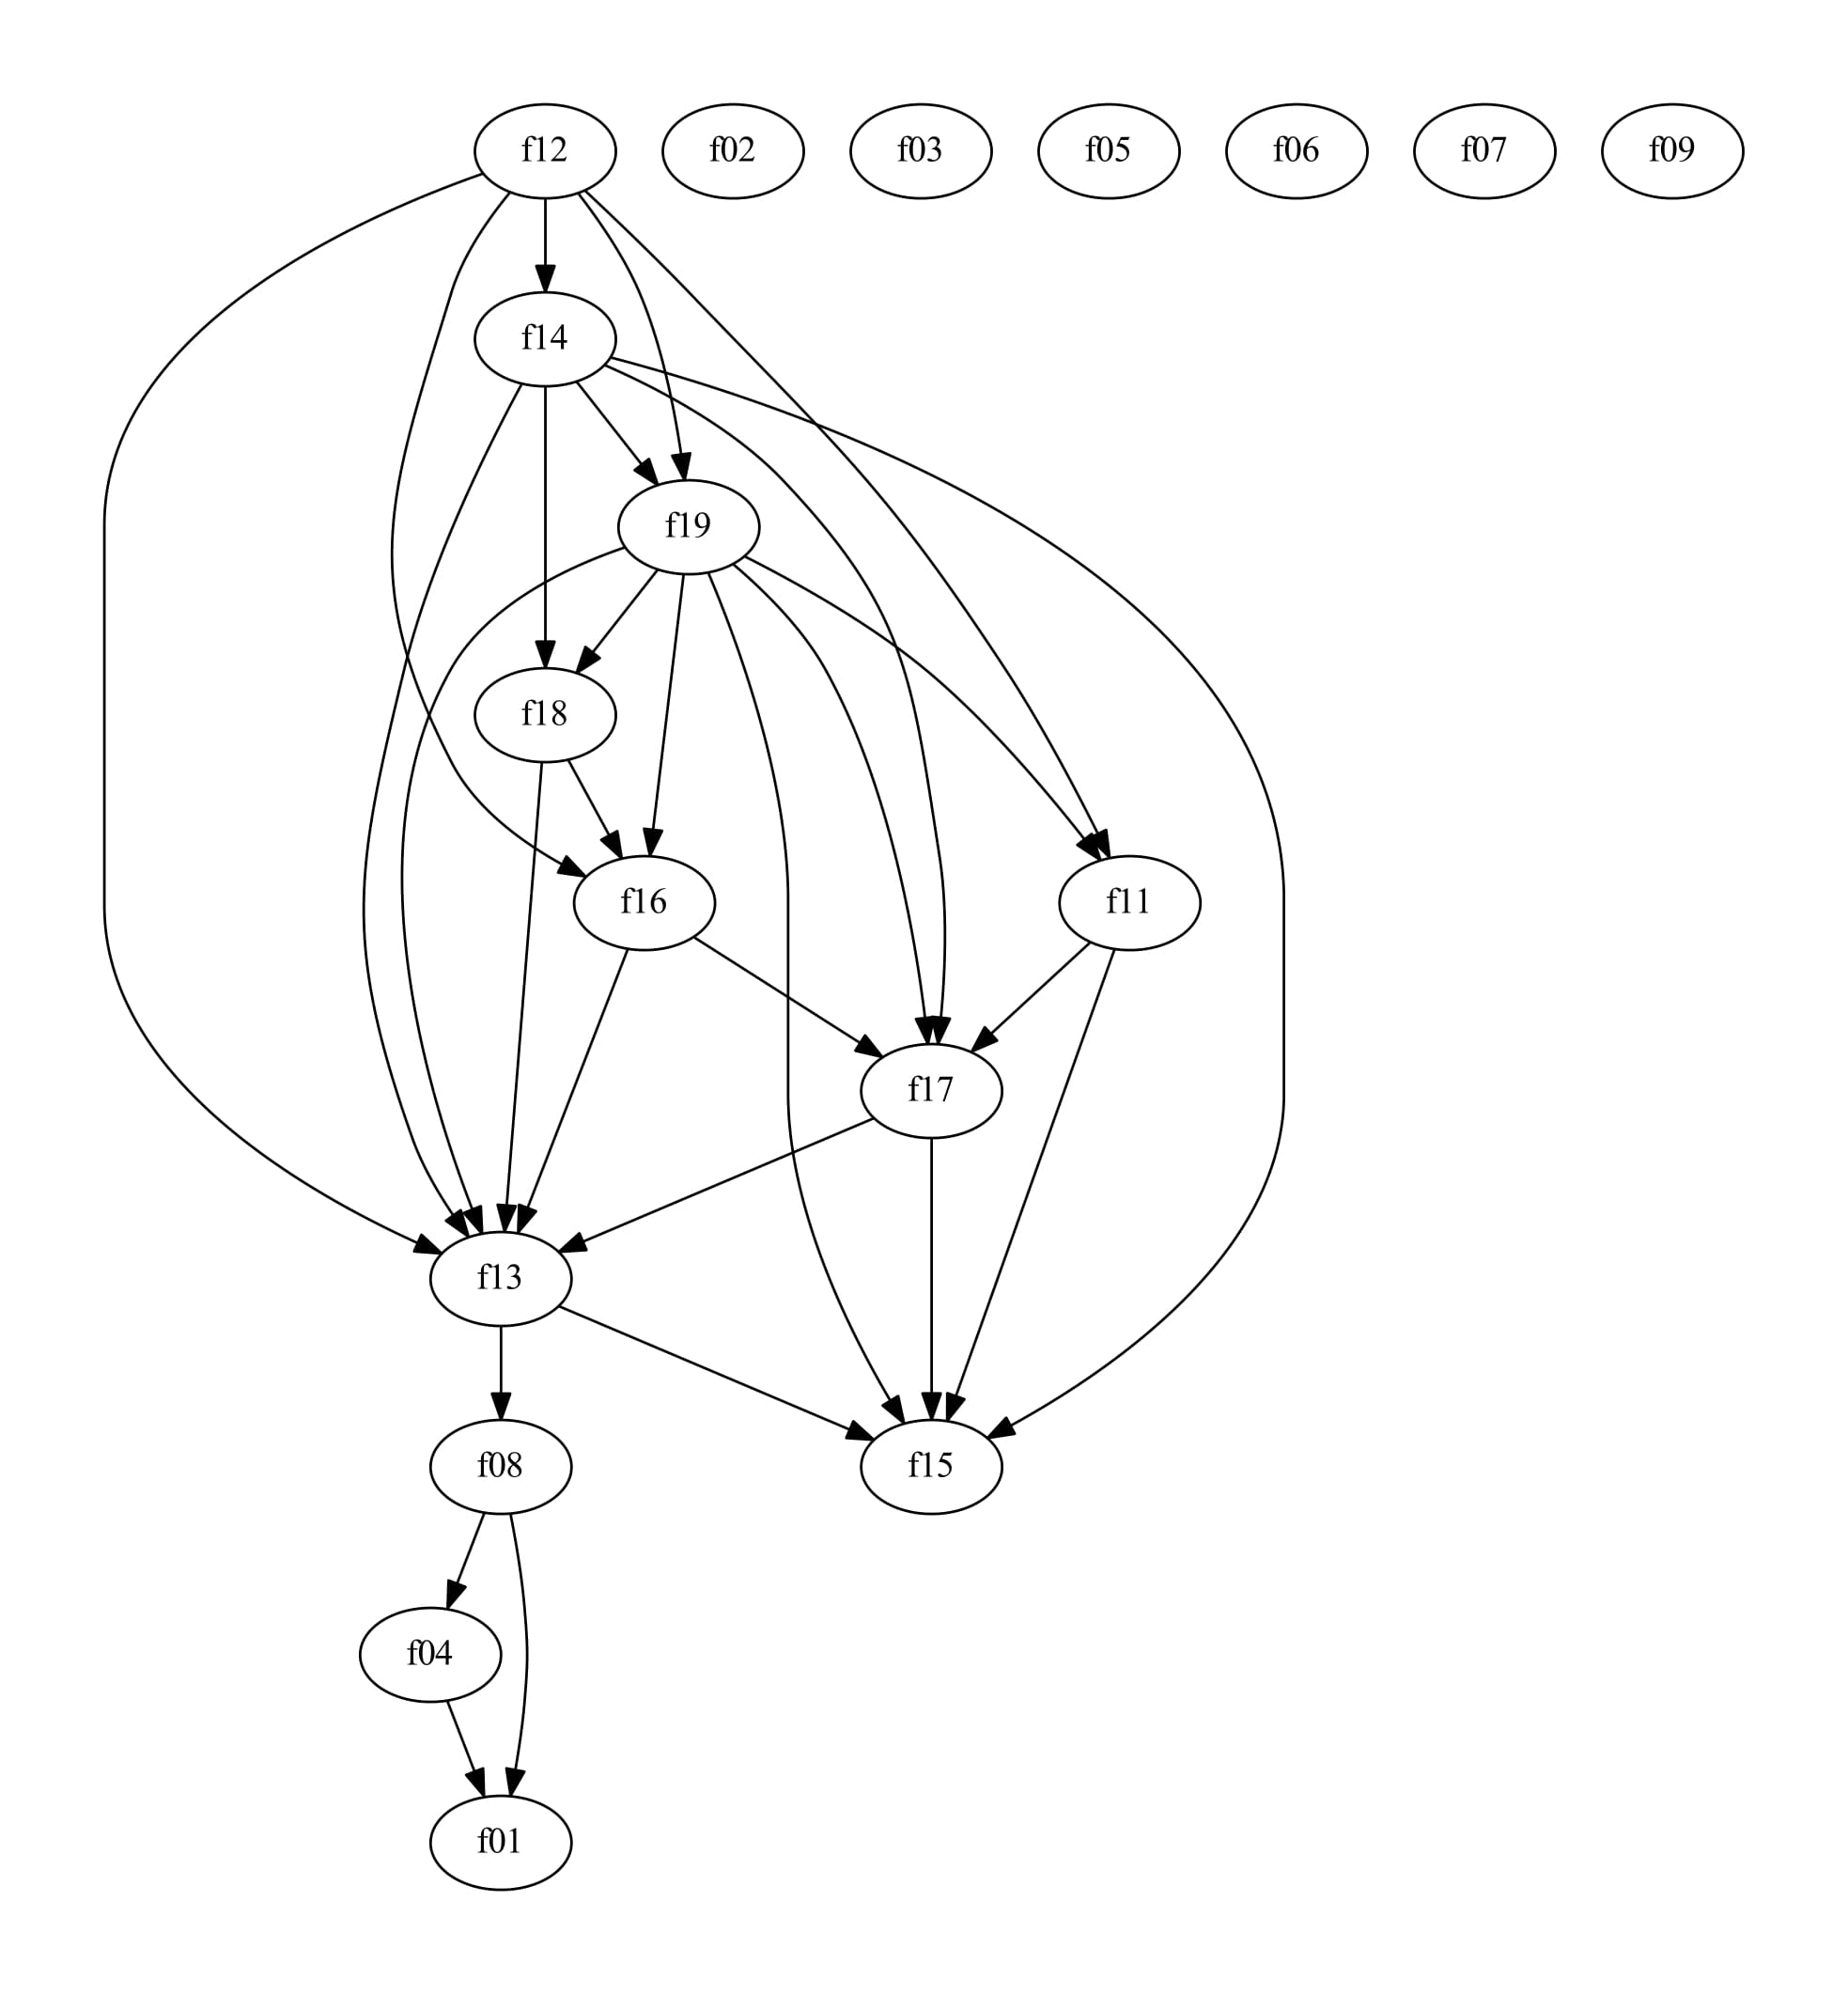
\includegraphics[width=50mm,scale=0.5]{bayesian_no_BD.jpg}
  \caption{Bayesian Network for Different Writer (BDeu Score)}
  \end{minipage}
\end{figure}
    \paragraph{BIC score:}
    Bayesian information criterion (BIC) or Schwarz criterion is a criterion for model selection among a finite set of models; the model with the lowest BIC is preferred. It is based, in part, on the likelihood function.When fitting models, it is possible to increase the likelihood by adding parameters, but doing so may result in overfitting. BIC attempts to resolve this problem by introducing a penalty term for the number of parameters in the model.\ [2] 
    
    \begin{figure}[h]
  \begin{minipage}{0.48\textwidth}
  \centering
  %\fbox{\rule[-.5cm]{0cm}{4cm} \rule[-.5cm]{4cm}{0cm}}
  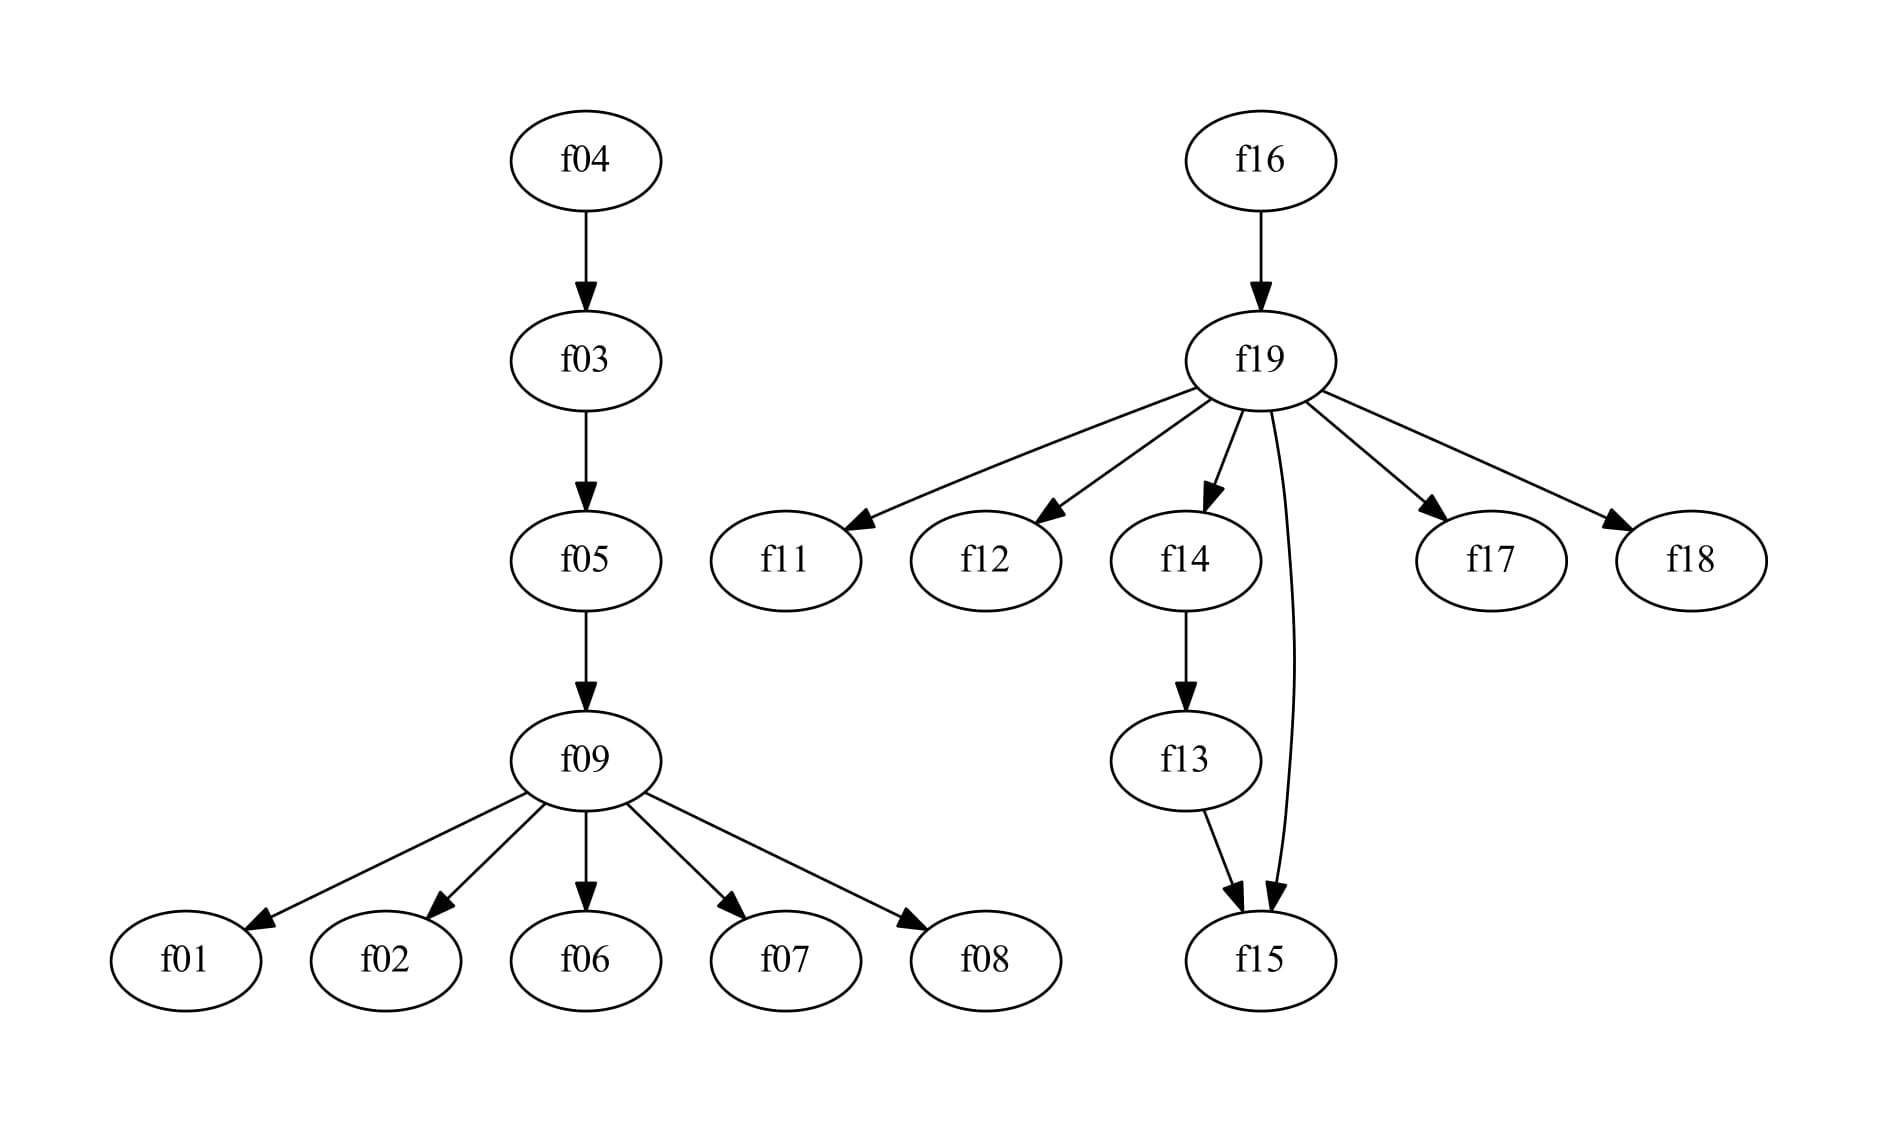
\includegraphics[width=50mm,scale=0.5]{bayesian_yes_BIC.jpg}
  \caption{Bayesian Network for Same Writer (BIC Score)}
  \end{minipage}\hfill
  \begin{minipage}{0.48\textwidth}
  \centering
  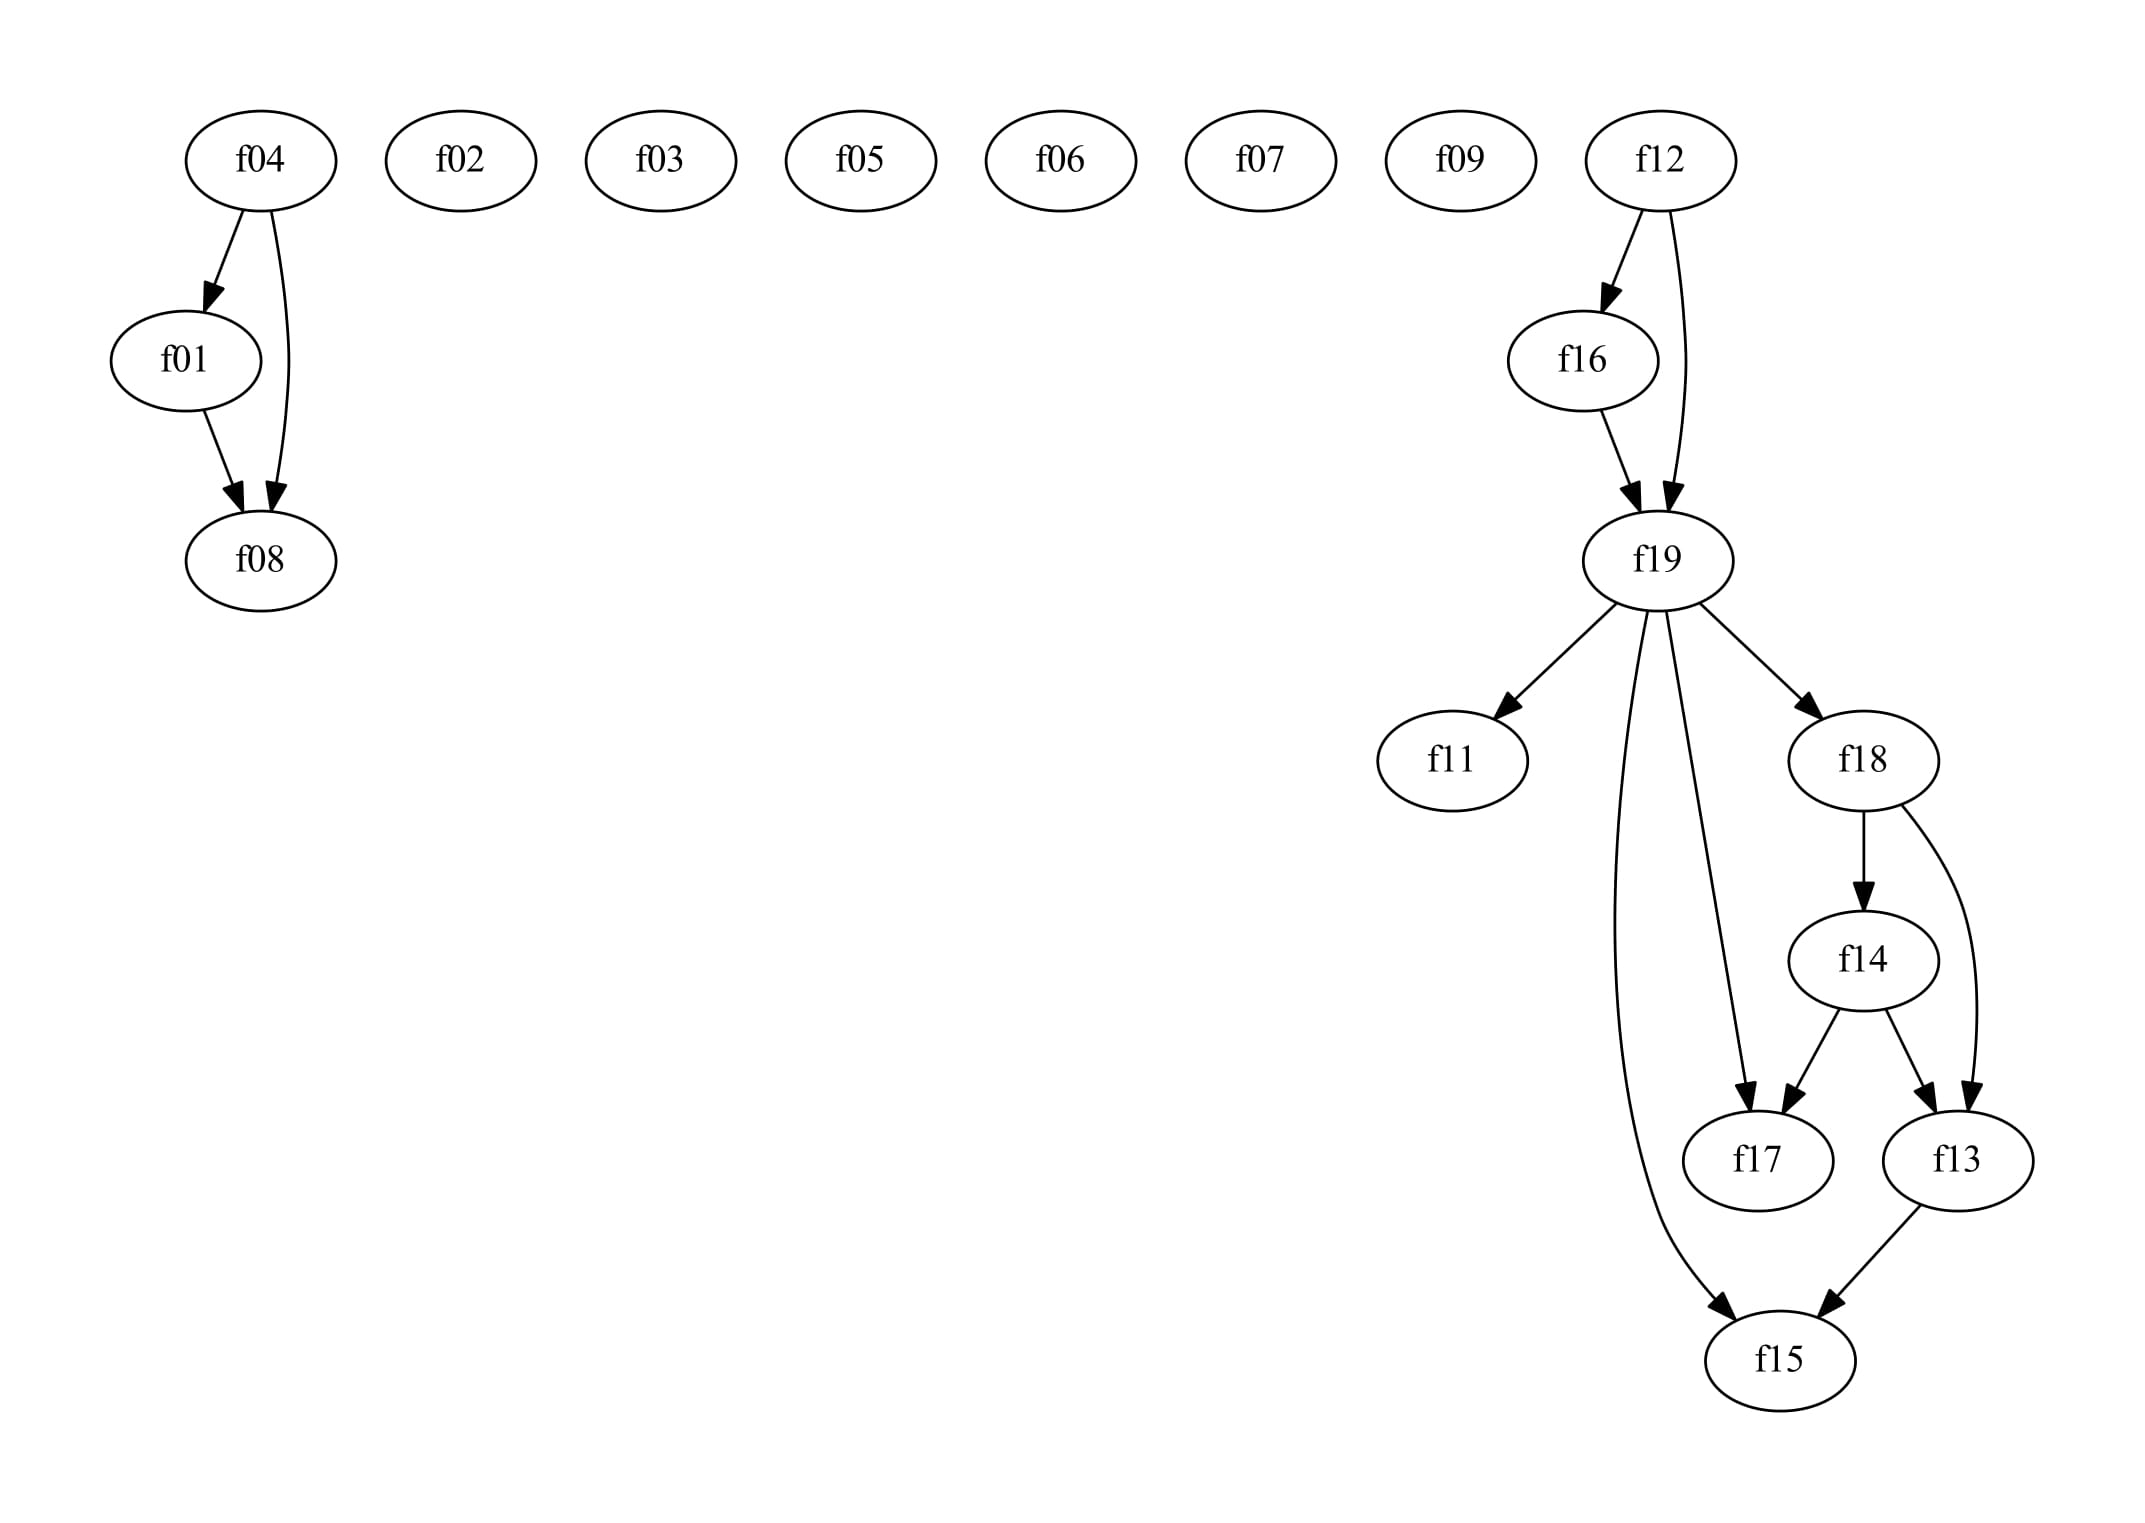
\includegraphics[width=50mm,scale=0.5]{bayesian_no_BIC.jpg}
  \caption{Bayesian Network for Different Writer (BIC Score)}
  \end{minipage}
\end{figure}
    
    \paragraph{K2 score:}
    The K2-score is a greedy search method, which incrementally adds a node to a parent set and finds the best parent set to maximize the joint probability of the structure and the database.\ [3]
    
    \begin{figure}[h]
  \begin{minipage}{0.48\textwidth}
  \centering
  %\fbox{\rule[-.5cm]{0cm}{4cm} \rule[-.5cm]{4cm}{0cm}}
  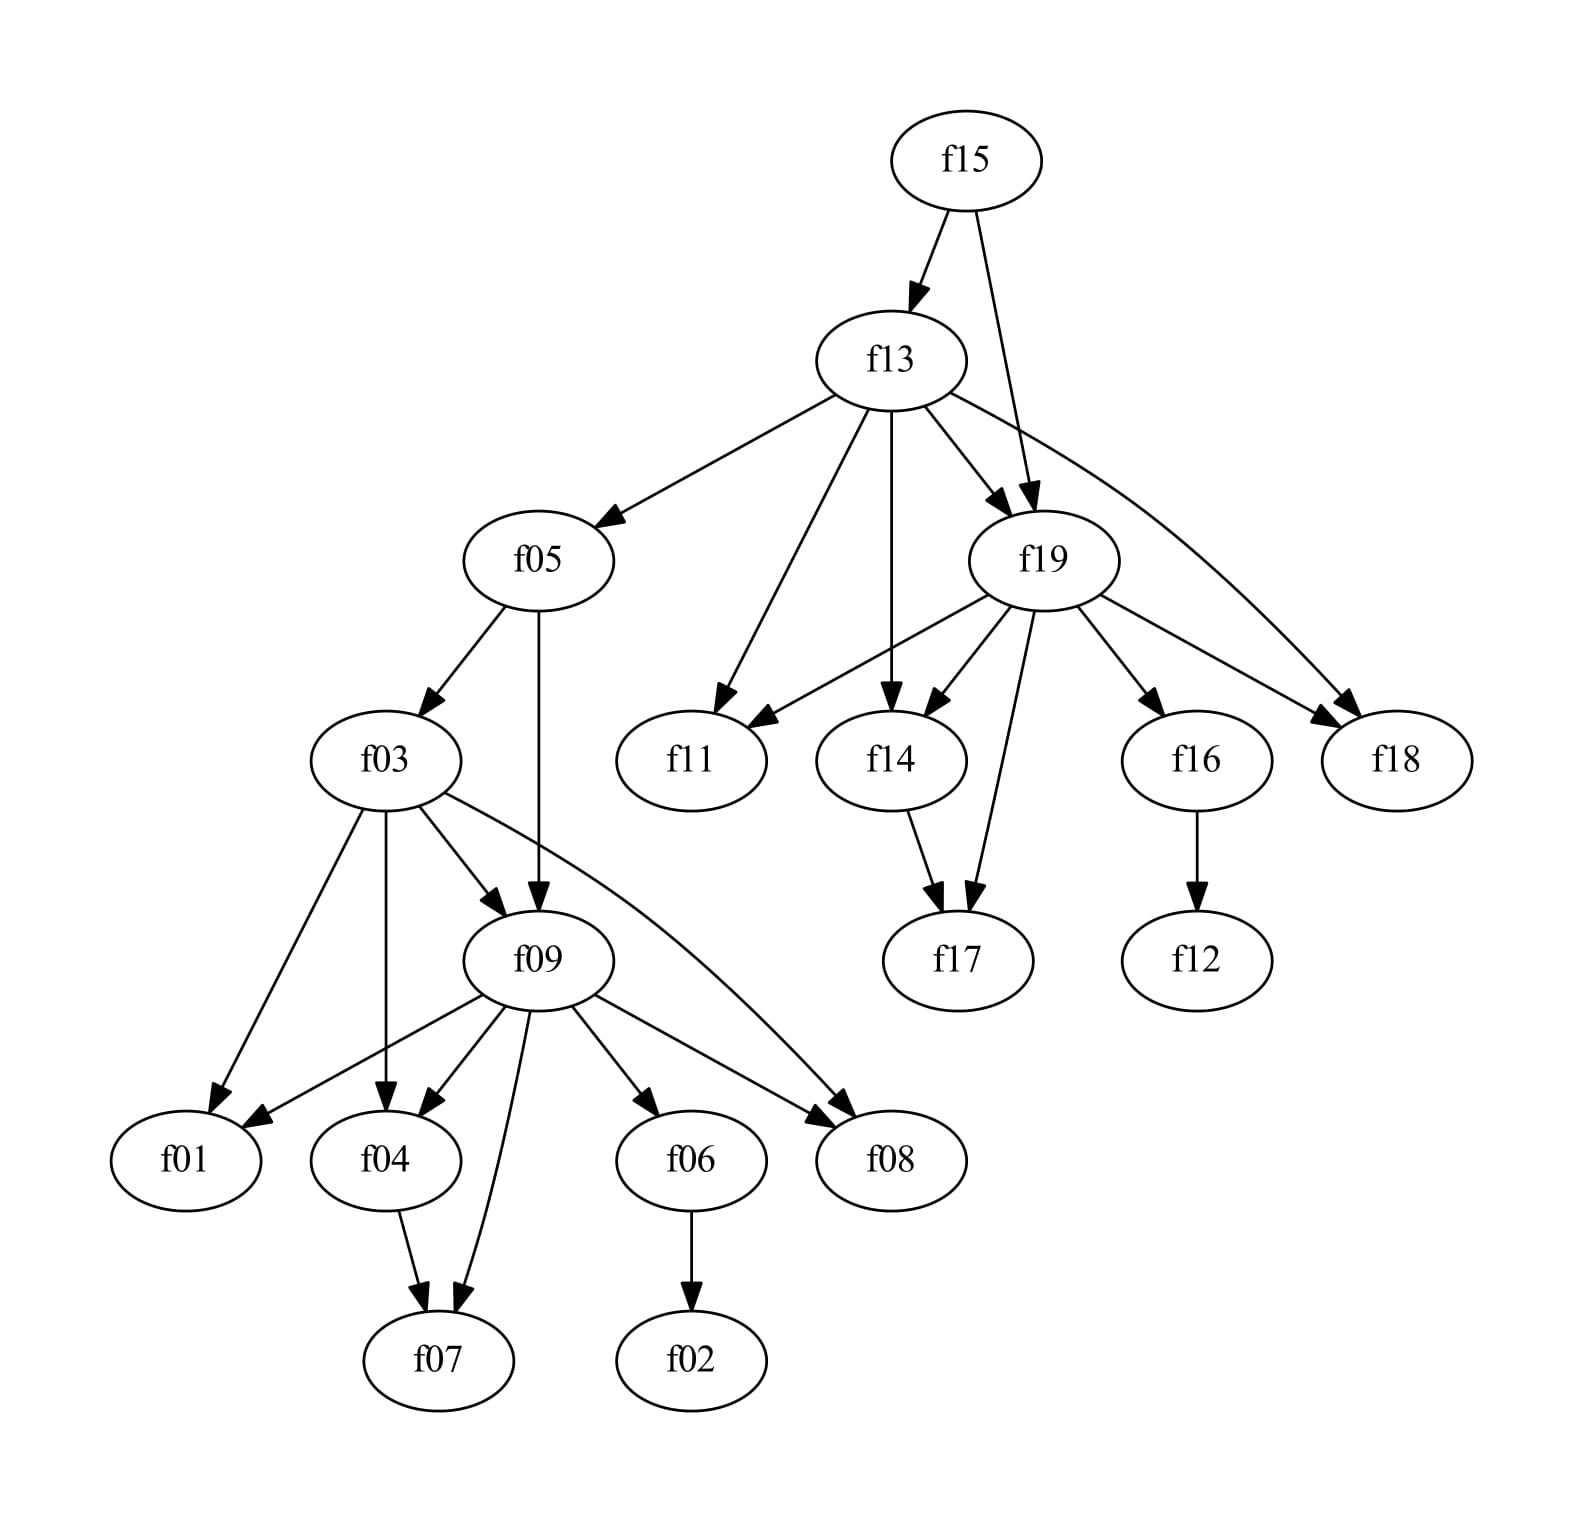
\includegraphics[width=50mm,scale=0.5]{bayesian_yes_K2.jpg}
  \caption{Bayesian Network for Same Writer (K2 Score)}
  \end{minipage}\hfill\hfill\hfill
  \begin{minipage}{0.48\textwidth}
  \centering
  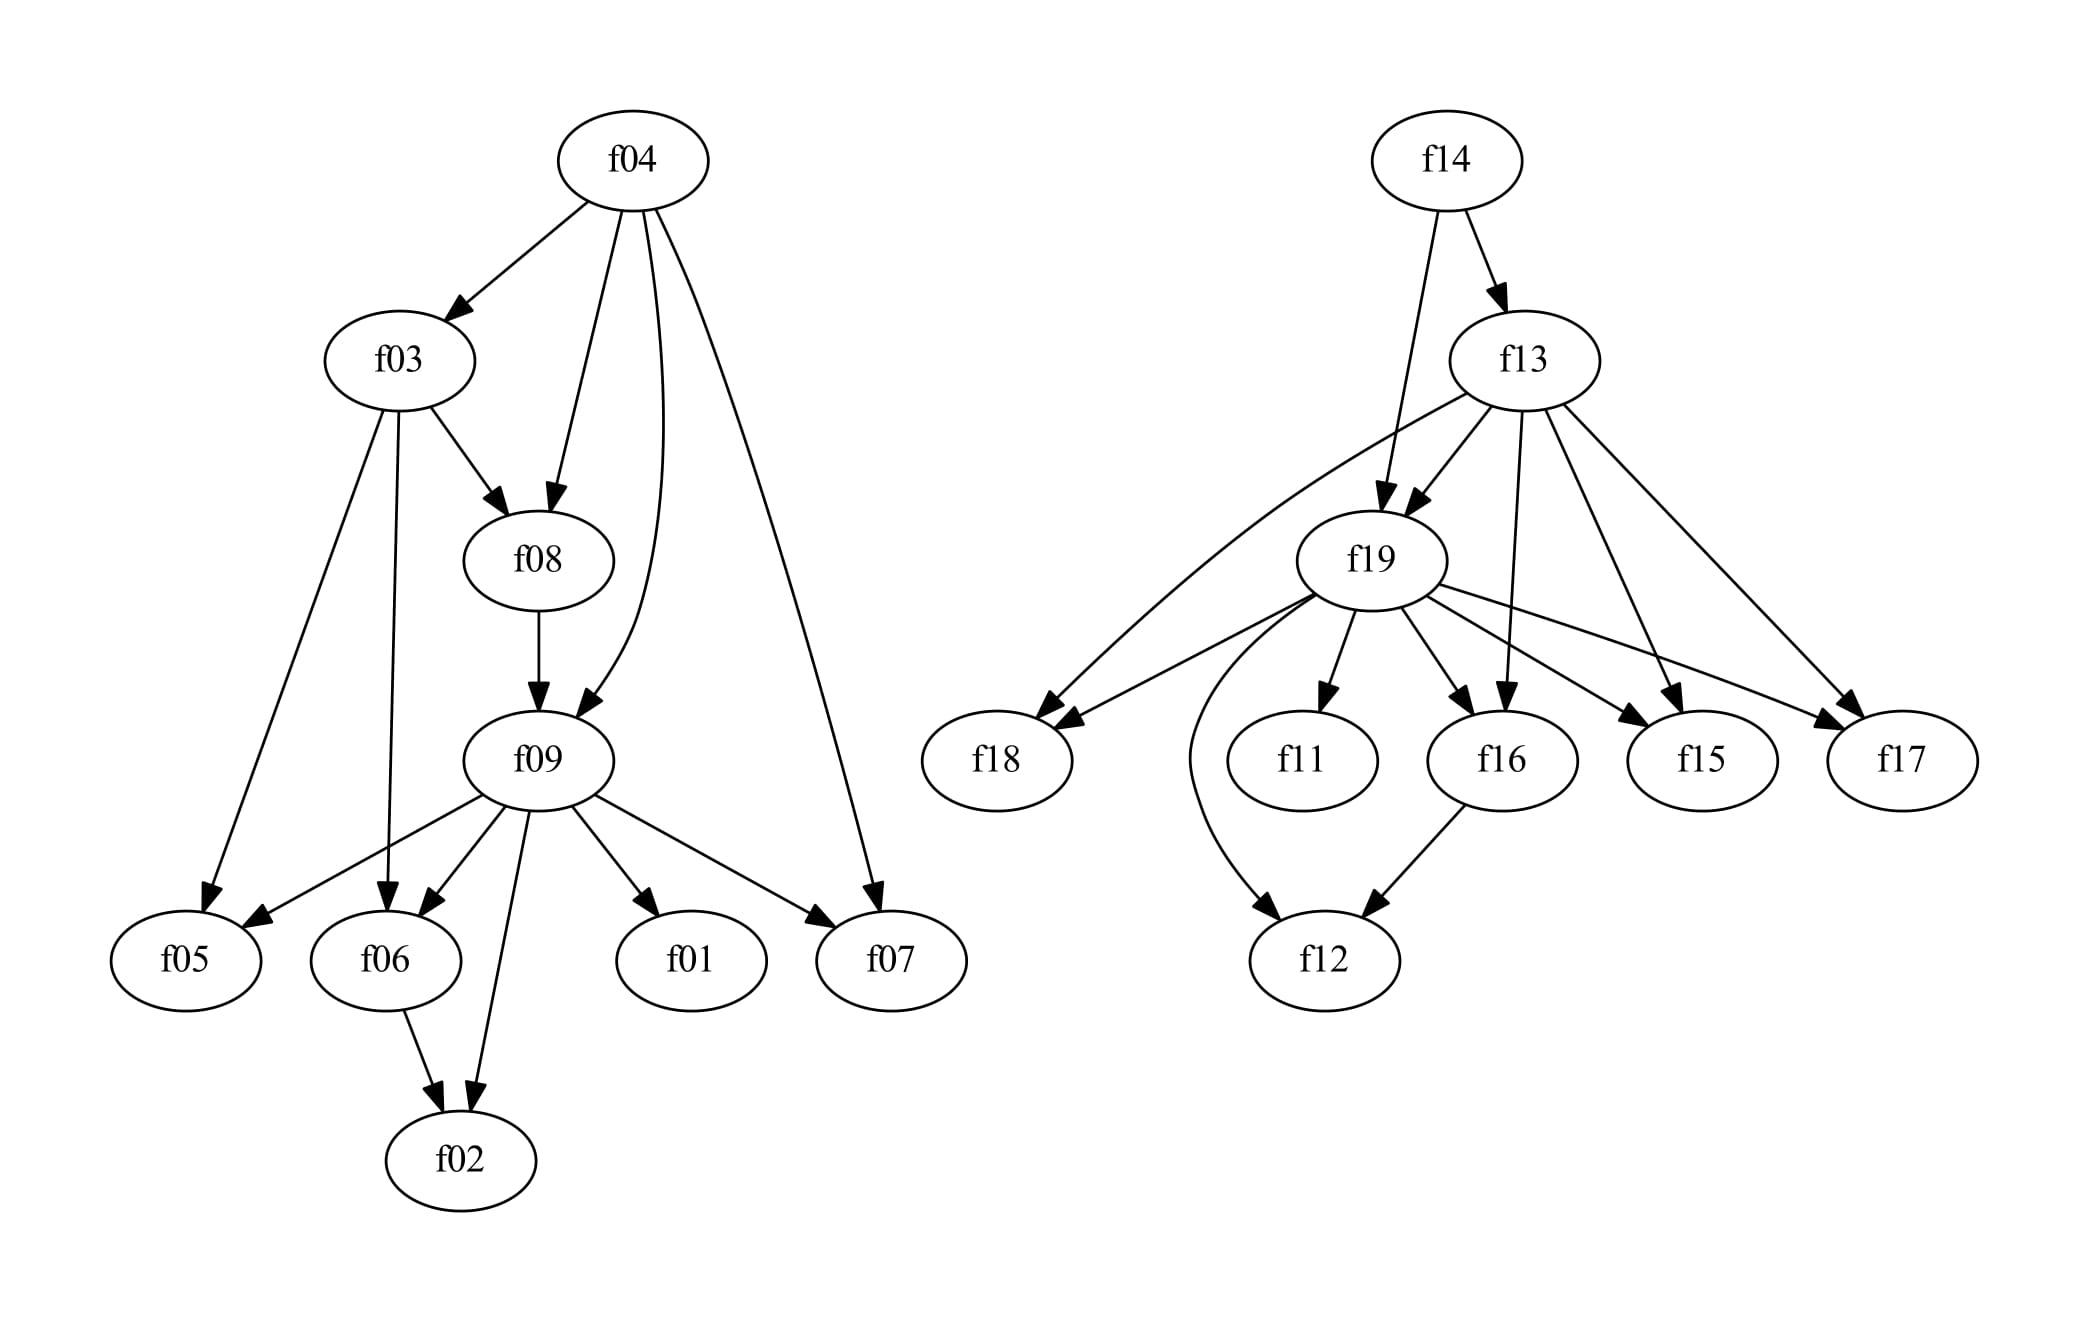
\includegraphics[width=50mm,scale=0.5]{bayesian_no_K2.jpg}
  \caption{Bayesian Network for Different Writer (K2 Score)}
  \end{minipage}
\end{figure}

    
    
    On each of these score estimators we performed local hill climbing search to find the Bayesian model that has optimal score with respect to the scoring method supplied in the constructor.\ [4]
    
    Out of all these models, it is found that K2 score estimator gives the most optimum model. Hence the final model used is the one found using K2 estimator.
    
    Using this model we get the joint probabilities from the product of CPDs for observed values of features. If log ratio of a given pair is positive, then the samples in the pair are considered to belong to the same writer else the samples belong to different writers.

\section{Simple Machine Learning}
\subsection{Dataset}
The dataset given for this approach consists of images of handwritten word \textit{'and'}. There are total 1568 writers and 15518 images in total written by the writers. 
 \subsubsection{PreProcessing}
        We arrange the given feature dataset in a hash-table like fashion where key is the writer number and value is a list of features of all those images where writer is the key(writer) 
    \subsubsection{Positive Pair Generation}
        For a writer we take two feature vectors in the value-space in the hashtable of the writer.Once first feature vector is chosen the other one is chosen at random to avoid choosing the exactly same feature vector twice.This is done for all writers.
    \subsubsection{Negative Pair Generation}
        We chose a writer and then we choosing a non-zero random increment, using this increment we choose another writer, and since the increment is non-zero we can not choose the same writer. We take any two feature vectors from these two writer as negative pair. We do this for all writers.
\subsection{Approach:}

\paragraph{Feature Extraction:\\}In this approach we have extracted SIFT features from the images and these features won't be of same length due to the nature of SIFT features and this will cause trouble from implementing neural network because it would require input of the same size to train on.\\ To tackle this problem we form an array of SIFT descriptors from all the images. Then we find the cluster centers using K-means [Note :  The number clusters specified will be the dimensionality of the feature vector] using the array of descriptors as data points and we store the centres in a file for later use. We can now cluster the data points according the centers obtained. The population of descriptors for an image in a cluster for every cluster forms the feature vector.\\
In simple words the feature vector is the histogram of population of descriptors for an image in each cluster.
\paragraph{Neural Network:\\}To determine whether given pair of features belongs to same writer or not we calculate the euclidean distance between the two feature vector and the network updates weights to decrease/increase this euclidean distance depending upon the known labels.If the features are from the same writer we try to decrease the distance otherwise we try to increase the distance.
For this updation we are making use of contrastive loss function which uses the following formula:\\

\begin{math}
\qquad \qquad L\big(W,Y,X_1,X_2\big)=\big(1-Y\big)\frac{1}{2}\big(D_w\big)^2 + \big(Y\big)\frac{1}{2}\big\{max\big(0,m- D_w\big)\big\}^2    \qquad[6]\\
\qquad \qquad  where\  D_w\  is\  the\  Euclidean\  distance\\
\end{math}\\
Since the labels are binary, in the above function only one part can be non-zero because other one has to be zero , this then changes weights in order to favour/hinder distance The objective of this architecture is not to classify input images, but to differentiate between them. So, a classification loss function (such as cross entropy) would not be the best fit. Instead, this architecture is better suited to use a contrastive function.[7] 

\subsection{Implementation:}
    We implement a Siamese network which learns the similarity of the two feature vectors.
    We use Keras library to handle all the gradient operations and model architecture. We concatenate the two inputs in a single vector one after the other and while calculating the distance we calculate the distance between first half and the second half this helps in keeping the model simple and to avoid two identical branches.
    The model architechture is as follows:
    \begin{figure}[h]
  \begin{minipage}{0.8\textwidth}
  \centering
  %\fbox{\rule[-.5cm]{0cm}{4cm} \rule[-.5cm]{4cm}{0cm}}
  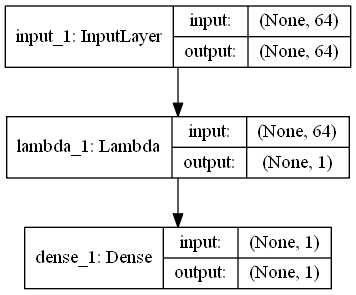
\includegraphics[scale=0.5]{model.png}
  \caption{Simple Machine Learning Model Architecture}
  \end{minipage}\hfill
  
\end{figure}
\section{Deep Siamese Network}
\subsection{Dataset:}
The dataset given is same as that used from simple machine learning which consists of 15518 images of handwritten word 'and',contributed by 1568 writers.
\subsubsection{PreProcessing}
        We arrange the given image dataset in a hash-table like fashion where key is the writer number and value is a list of features of all those images where writer is the key(writer) 
    \subsubsection{Positive Pair Generation}
        For a writer we take two images in the value-space in the hashtable of the writer.Once first feature vector is chosen the other one is chosen at random to avoid choosing the exactly same feature vector twice.This is done for all writers.
    \subsubsection{Negative Pair Generation}
        We chose a writer and then we choosing a non-zero random increment, using this increment we choose another writer, and since the increment is non-zero we can not choose the same writer. We take any two images from these two writer as negative pair. We do this for all writers.
        
\subsection{Approach:}
For deep learning approach, we are going to make use of Siamese Architechture Since the problem requires to compare 2 samples of images and determine whether they belong to the same writer we are going to use Siamese Neural Network. We have two branches of  Convolutional Neural Network which will work as automatic feature extractors and the outputs of these sister branches are then merged in lambda layer of Euclidean Distance and to determine whether the two samples belong to same writer or not. A contrastive loss function is used to update weights in order to favour/hinder the distance observed.\\

\begin{math}
\qquad \qquad L\big(W,Y,X_1,X_2\big)=\big(1-Y\big)\frac{1}{2}\big(D_w\big)^2 + \big(Y\big)\frac{1}{2}\big\{max\big(0,m- D_w\big)\big\}^2    \qquad[6]
\end{math}

\subsection{Implementation:}
 
\paragraph{Siamese Neural Network:}
A Siamese networks consists of two identical convolutional neural networks, each taking one of the two input images. The output of the two networks are then fed to a euclidean distance function , which calculates the similarity between the two images.The loss function to update weights is the contrastive loss function
There are two sister networks, which are identical neural networks, with the exact same weights.
Each image in the image pair is fed to one of these networks.[7]

\paragraph{Contrastive Loss Function:}
The objective of the siamese architecture is not to classify input images, but to differentiate between them. So, a classification loss function (such as cross entropy) would not be the best fit. Instead, this architecture is better suited to use a contrastive function. Intuitively, this function just evaluates how well the network is distinguishing a given pair of images.[7]

In this approach for feature extraction, we are making use of Convolutional Neural Network

\paragraph{Convolutional Neural Network:}
Convolutional Neural Networks are very similar to ordinary Neural Networks they are made up of neurons that have learnable weights and biases. Each neuron receives some inputs, performs a dot product and optionally follows it with a non-linearity.The whole network still expresses a single differentiable score function: from the raw image pixels on one end to class scores at the other. A simple CNN is a sequence of layers, and every layer of a CNN transforms one volume of activations to another through a differentiable function. There are  three main types of layers used to build CNN architectures: Convolutional Layer, Pooling Layer, and Fully-Connected Layer.Convolutional layer will compute the output of neurons that are connected to local regions in the input, each computing a dot product between their weights and a small region they are connected to in the input volume.Pooling layer will perform a downsampling operation along the spatial dimensions (width, height).
Finally the fully connected layer gives the class score, thereby deciding whether given sample belongs to the same writer or not. [8]

\begin{figure}[H]
  \centering
  %\fbox{\rule[-.5cm]{0cm}{4cm} \rule[-.5cm]{4cm}{0cm}}
  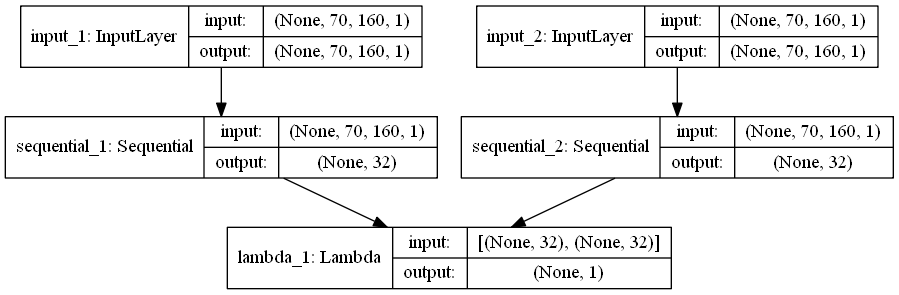
\includegraphics[scale= 0.4]{siamese_dl.png}
  \caption{Deep Siamese Model Architecture}
  
\end{figure}

\section{Conclusion}
 We can see from the graph [Figure 8] and the table below that the approach involving Deep Siamese Network yeilds the best results. But it should be also considered the the Deep Learning model required a lot more of computation power than the other approaches. The PGM approach required the least computation power (excluding Bayesian Structure Learning as that can done manually).
Overall the simple machine learning model's performance was in the Goldilock's zone as it's accuracy is also reasonable and it didn't require much computing power. \\
\begin{table}[!htb]
  \caption{Accuracies of each method}
  \label{sample-table}
  \centering
  \begin{tabular}{ll}           \\
    \cmidrule{1-2}
    Approach     & Accuracy \\
    \midrule
    PGM [ Mulinet ] & 54.15\%\\
    Simple Machine Learning      & 63.23\%\\
    Deep Siamese Network     & 82.53\%      \\
    \bottomrule
  \end{tabular}
\end{table}
\begin{figure}[H]
  \centering
  %\fbox{\rule[-.5cm]{0cm}{4cm} \rule[-.5cm]{4cm}{0cm}}
  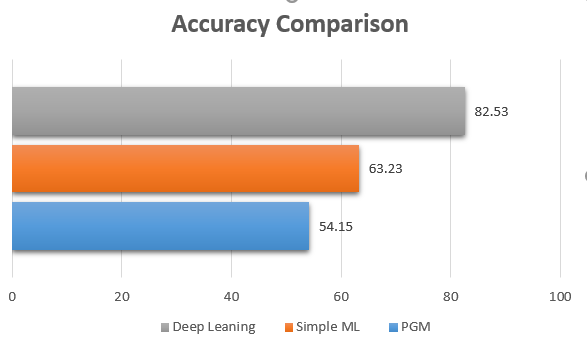
\includegraphics{accuracycomparison.png}
  \caption{Accuracy}
  
\end{figure}







\section*{Acknowledgments:}
We are thankful to Professor Sargur N. Srihari and teaching assistants, Mihir Chauhan and Mohammad Shaikh for giving us this opportunity and guiding us throughout the course of the project.

\section*{References}

[1]\ Mauro Scanagatta, Cassio P. de Campos, and Marco Zaffalon \textit{Min-BDeu and Max-BDeu Scores for Learning
Bayesian Networks}

[2]\  \url{https://en.wikipedia.org/wiki/Bayesian_information_criterion}

[3]\  Shulin Yang and Kuo-Chu Chang \textit{Comparison of Score Metrics for Bayesian Network learning }

[4]\  \url{http://pgmpy.org/estimators.html#hill-climb-search}

[5]\  \url{https://arxiv.org/ftp/arxiv/papers/1303/1303.5718.pdf}

[6]\ Raia Hadsell, Sumit Chopra, Yann LeCun \textit{Dimensionality Reduction by Learning an Invariant Mapping},The Courant Institute of Mathematical Sciences,New York University, 719 Broadway, New York, NY 1003, USA. 

[7]\ \url{https://hackernoon.com/one-shot-learning-with-siamese-networks-in-pytorch-8ddaab10340e}
[8]\ \url{http://cs231n.github.io/convolutional-networks/}
\end{document}
